%encoding:utf-8

\documentclass{beamer}

\usepackage{polski}
\usepackage[utf8]{inputenc}
\usepackage{hyperref}
\usepackage{color}
\usepackage{graphicx}
\usepackage{listings}

\usetheme{default}
\usecolortheme{beaver}
\setbeamercolor{title}{bg=white}
\definecolor{forestgreen}{HTML}{009B55}

\title{Ruby extensions in C}
\author{Paweł Placzyński}
\institute{Ragnarson}

\begin{document}
  \frame{\titlepage}

  \begin{frame}
    \begin{center}
      \href{https://github.com/placek}{github.com/placek}


      \href{https://facebook.com/placzynski.pawel}{facebook.com/placzynski.pawel}
    \end{center}
  \end{frame}

  \begin{frame}
    \frametitle{Ruby vs. C}
    \begin{columns}[c]
      \column{.5\textwidth}
        {\centering \large Ruby}
      \column{.5\textwidth}
        {\centering \large C}
    \end{columns}
    \begin{columns}[t]
      \column{.5\textwidth}
        \only<1-> {
        \begin{itemize}
          \item \color{forestgreen} prostota składni, intuicyjność
          \item \color{forestgreen} lukier składniowy
          \item \color{forestgreen} duck typing, programowanie funkcyjne, programowanie imperatywne, metaprogramowanie
        \end{itemize}}
      \column{.5\textwidth}
        \only<3-> {
        \begin{itemize}
          \item \color{forestgreen} kontrola wykonywanych poleceń (niskopoziomowość)
          \item \color{forestgreen} wydajność !!!
        \end{itemize}}
    \end{columns}
    \begin{columns}[t]
      \column{.5\textwidth}
        \only<2-> {
        \begin{itemize}
          \item \color{red} ,,zasobożerność''
          \item \color{red} wydajność
        \end{itemize}}
      \column{.5\textwidth}
        \only<4-> {
        \begin{itemize}
          \item \color{red} łatwo o pomyłkę
          \item \color{red} nieczytelny kod
          \item \color{red} nie intuicyjne zachowanie
        \end{itemize}}
    \end{columns}
  \end{frame}

  \begin{frame}
    \frametitle{Ruby vs. C}
    \begin{center}
      {\large {\color{gray} \textit{,,Ruby jest prosty z wyglądu, ale bardzo skomplikowany w środku, tak jak ciało ludzkie.''}\\\hfill - - Matz}}
    \end{center}
  \end{frame}

  \begin{frame}
    \frametitle{Ruby vs. C}
    \begin{center}
      \href{http://benchmarksgame.alioth.debian.org/u64q/benchmark.php?lang=yarv\&lang2=gcc}{benchmarksgame.alioth.debian.org}
    \end{center}
  \end{frame}

  \begin{frame}
    \frametitle{Ruby vs. C}
    \begin{center}
      \begin{figure}[h!]
        \caption{Porównanie języka Ruby z językiem C.}
        \centering
          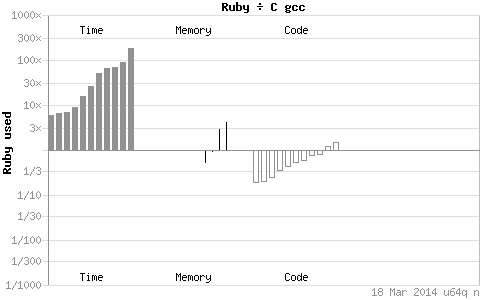
\includegraphics[width=0.8\textwidth]{img/chartvs.png}
      \end{figure}
    \end{center}
  \end{frame}

  \begin{frame}
    \frametitle{Algorytm Levenshtein'a -- definicja}
    \textbf{Odległością} pomiędzy dwoma napisami jest najmniejsza liczba działań prostych, przeprowadzających jeden napis na drugi. \\~\\
    \textbf{Działaniem prostym} na napisie nazwiemy:
    \begin{itemize}
      \item wstawienie nowego znaku do napisu,
      \item usunięcie znaku z napisu,
      \item zamianę znaku w napisie na inny znak.
    \end{itemize}
  \end{frame}

  \begin{frame}
    \frametitle{Algorytm Levenshtein'a -- przykład}
    \begin{center}
      \only<1-> {\LARGE foka}


      \only<2-> {$\downarrow$}


      \only<2-> {\LARGE {\color{red}k}oka}


      \only<3-> {$\downarrow$}


      \only<3-> {\LARGE ko{\color{red}t}ka \\~\\}
      \only<4-> {\normalsize dwa proste działania -- odległość równa 2}
    \end{center}
  \end{frame}

  \begin{frame}
    \frametitle{Algorytm Levenshtein'a -- więcej informacji}
    \begin{center}
      \href{http://pl.wikipedia.org/wiki/Odleg\%C5\%82o\%C5\%9B\%C4\%87\_Levenshteina}{pl.wikipedia.org/wiki/Odległość\_Levenshteina} \\~\\
      \href{http://www.algorytm.org/przetwarzanie-tekstu/odleglosc-levenshteina-odleglosc-edycyjna.html}{www.algorytm.org/przetwarzanie-tekstu/odleglosc-levenshteina-odleglosc-edycyjna.html}
    \end{center}
  \end{frame}

  \begin{frame}
    \frametitle{Benchmark}
    \begin{center}
      \begin{itemize}
        \item przykładowy tekst z \href{http://lipsum.com/}{lipsum.com}
        \item próbki: 100, 200, 300, \ldots, 700 słów
        \item kombinacja (bez powtórzeń) dwóch słów z próbki
        \item obliczenie odległości Levenshtein'a dla każdej pary słów
      \end{itemize}
    \end{center}
  \end{frame}

  \begin{frame}
    \frametitle{Benchmark -- czysty Ruby}
    \begin{center}
      \lstinputlisting[firstline=1, lastline=17, basicstyle=\footnotesize]{benchmark_results.txt}
    \end{center}
  \end{frame}

  \begin{frame}
    \frametitle{Benchmark -- rozszerzenie Ruby w języku C}
    \begin{center}
      \lstinputlisting[firstline=19, lastline=35, basicstyle=\footnotesize]{benchmark_results.txt}
    \end{center}
  \end{frame}

\end{document}
